\section{Results}

\begin{sansmath}
\sessionpy{pytex_subfigs(
        [
                {'script':'scripts/taskgroup.py', 'conf':'article/3x1.conf', 'options_pre':'{.322\\textwidth}',
                        'caption':'Task group comparison for animals targeted at all explored combinations of implant coordinates.',
                        'label':'mvt',
                        },
                {'script':'scripts/implant_coordinates_block.py', 'conf':'article/3x1_coordinates.conf', 'options_pre':'{.322\\textwidth}',
                        'caption':'Implant coordinate comparison for block stimulation trials (inner dots indicate best category group).',
                        'label':'mvib',
                        },
                {'script':'scripts/implant_coordinates_phasic.py', 'conf':'article/3x1_coordinates.conf', 'options_pre':'{.322\\textwidth}',
                        'caption':'Implant coordinate comparison for phasic stimulation trials (inner dots indicate best category group).',
                        'label':'mvip',
                        },
                ],
        caption='
                \\textbf{Sensitivity of VTA activation to stimulation protocol category and implant coordinates.}
                Depicted are multifactorial (protocol and operative feature) comparisons of signal intensity in the VTA region of interest.
                ',
        label='fig:mv',
        )}
\end{sansmath}

\begin{sansmath}
\sessionpy{pytex_subfigs(
        [
                {'script':'scripts/map_block_filtered_controlled.py', 'label':'subjects', 'conf':'article/2x1_map.conf', 'options_pre':'{.48\\textwidth}',
                        'caption':'Slices centered on VTA. \\vspace{-.2em}',
                        'label':'filtered_map',
                        },
                {'script':'scripts/map_block_filtered_controlled_auto.py', 'label':'subjects', 'conf':'article/2x1_map.conf', 'options_pre':'{.48\\textwidth}',
                        'caption':'Slices centered on largest cluster. \\vspace{-.2em}',
                        'label':'filtered_mapa',
                        },
                {'script':'scripts/distributions_block_filtered_controlled.py', 'label':'tasks', 'conf':'article/distributions.conf', 'options_pre':'{.95\\textwidth}',
                        'caption':'Distribution densities of t-statistic values in the 10 most strongly activated areas.',
                        'label':'filtered_dist',
                        },
                ],
        caption='
                \\textbf{Block stimulation elicits strong and clustered activity in the ventral striatum, particularly the nucleus accumbens.}
                Depicted are the results of the second-level analysis for block stimulus evoked activity observed in the best implant group animals, and corrected for the negative control baseline.
                The figures show volumetric population t-statistic maps \\textbf{(\subref{fig:filtered_map}, \subref{fig:filtered_mapa})} thresholded at $\mathrm{t \geq 3}$, as well as a break-down of activation along atlas parcellation regions \\textbf{(\subref{fig:filtered_dist})}.
                ',
        label='fig:filtered',
        options_pre='\\centering',
        )}
\end{sansmath}

\begin{sansmath}
\sessionpy{pytex_subfigs(
        [
                {'script':'scripts/map_block_other_controlled.py', 'label':'subjects', 'conf':'article/2x1_map.conf', 'options_pre':'{.48\\textwidth}',
                        'caption':'Slices centered on VTA. \\vspace{-.2em}',
                        'label':'other_map',
                        },
                {'script':'scripts/map_block_other_controlled_auto.py', 'label':'subjects', 'conf':'article/2x1_map.conf', 'options_pre':'{.48\\textwidth}',
                        'caption':'Slices centered on largest cluster. \\vspace{-.2em}',
                        'label':'other_mapa',
                        },
                {'script':'scripts/distributions_block_other_controlled.py', 'label':'tasks', 'conf':'article/distributions.conf', 'options_pre':'{.95\\textwidth}',
                        'caption':'Distribution densities of t-statistic values in the 10 most strongly activated areas.',
                        'label':'other_dist',
                        },
                ],
        caption='
                \\textbf{In the rejected implant category group, stimulus evoked activity in response to block stimulation is reduced and differently distributed.}
                Depicted are results of the second-level analysis for block stimulus evoked activity observed in the rejected implant group animals, and corrected for the negative control baseline.
                The figures show volumetric population t-statistic maps \\textbf{(\subref{fig:other_map}, \subref{fig:other_mapa})} thresholded at $\mathrm{t \geq 3}$, as well as a break-down of activation along atlas parcellation regions \\textbf{(\subref{fig:other_dist})}.
                ',
        label='fig:other',
        options_pre='\\centering',
        )}
\end{sansmath}

\begin{sansmath}
\sessionpy{pytex_subfigs(
        [
                {'script':'scripts/map_features_filtered.py', 'conf':'article/2asymetric_map.conf',
                        'options_pre':'{.39\\textwidth}',
                        'options_pre_caption':'\\vspace{.5em}',
                        'caption':'Contrast between VTA functional activation and structural projections, showing slices centered on largest cluster, statistical map thresholded at $\mathrm{3 \geq t \geq 3}$. \\vspace{.8em}',
                        'label':'mff',
                        },
                {'script':'scripts/distributions_features_filtered.py', 'conf':'article/2asymetric_distributions.conf',
                        'options_pre':'{.595\\textwidth}\\vspace{-1.55em}',
                        'options_pre_caption':'\\vspace{-1.5em}',
                        'caption':'Distribution densities of t-statistics, showing the regions were VTA functional activation exceedes structural projections most strongly. As seen in \\textbf{(\subref{fig:mff})}, structural projection only sparsely exceedes functional activation (distributions under \\textbf{\cref{fig:dffn}}).\\vspace{.8em}',
                        'label':'dff',
                        },
                {'script':'scripts/features_filtered_coronal.py', 'conf':'article/coronal.conf', 'options_pre':'{.99\\textwidth}',
                        'caption':'
                                Coronal slice overlay, showing the VTA functional activation t-statistic heatmap (as in \\textbf{\\cref{fig:filtered}}), and the VTA structural projection outline, both thresholded at $\mathrm{3 \geq t \geq 3}$.
                                ',
                        'options_post':'\\vspace{1.2em}',
                        'label':'ffc',
                        },
                {'script':'scripts/features_correlation_rois.py', 'conf':'article/1col.conf', 'options_pre':'{.48\\textwidth}',
                        'caption':'
                                Region-wise regression plot between functional and structural projection maps (same as iin \\textbf{\subref{fig:ffc}}).
                                Tinted area indicates the \\SI{99}{\percent} confidence interval of the regression estimate.
                                ',
                        'options_pre_caption':'\\vspace{-1.5em}',
                        'label':'fcr',
                        'figure_format':'pdf',
                        },
                {'script':'scripts/features_correlation_voxels.py', 'conf':'article/1col_with_margins.conf', 'options_pre':'{.48\\textwidth}',
                        'caption':'
                                Voxel-wise regression plot between functional and structural projection maps (same as in \\textbf{\subref{fig:ffc}}).
                                Tinted area indicates the \\SI{99}{\percent} confidence interval of the regression estimate.
                                ',
                        'options_pre_caption':'\\vspace{-1.5em}',
                        'label':'fcv',
                        'figure_format':'pdf',
                        },
                ],
        caption='
                \\textbf{Comparing VTA functional activation to structural projection data reveals broadly similar patterns, with differences in the contralateral and the dorsal ipsilateral striatum.}
                Depicted are contrast statistic values, taking into account variability across subjects \\textbf{(\subref{fig:mff}, \subref{fig:dff})}, alongside an overlay \\textbf{(\subref{fig:ffc})} and correlation analyses \\textbf{(\subref{fig:fcr}, \subref{fig:fcv})} of the the population-level functional and structural statistic maps.
                ',
        label='fig:f',
        options_pre='\\centering\n\\vspace{-2em}',
        )}
\end{sansmath}

\begin{sansmath}
\sessionpy{pytex_subfigs(
        [
                {'script':'scripts/map_block_filtered_seed.py', 'label':'subjects', 'conf':'article/2x1_map.conf', 'options_pre':'{.48\\textwidth}',
                        'caption':'Slices centered on the VTA annotation (delineated in pink). \\vspace{-.2em}',
                        'label':'seed_map',
                        },
                {'script':'scripts/map_block_filtered_seed_auto.py', 'label':'subjects', 'conf':'article/2x1_map.conf', 'options_pre':'{.48\\textwidth}',
                        'caption':'Slices centered on largest cluster. \\vspace{-.2em}',
                        'label':'seed_mapa',
                        },
                {'script':'scripts/distributions_block_filtered_seed.py', 'label':'tasks', 'conf':'article/distributions.conf', 'options_pre':'{.95\\textwidth}',
                        'caption':'Distribution densities in the 10 regions with the highest functional connectivity to the VTA seed.',
                        'label':'seed_dist',
                        },
                ],
        caption='
                \\textbf{VTA seed-based functional connectivity shows a primary projection weighting towards the right nucleus accumbens.}
                Depicted are volumetric population t-statistic maps \\textbf{(\subref{fig:seed_map}, \subref{fig:seed_mapa})} thresholded at $\mathrm{t \geq 3}$, as well as a break-down of activation along atlas parcellation regions \\textbf{(\subref{fig:seed_dist})}.
                ',
        label='fig:seed',
        options_pre='\\centering',
        )}
\end{sansmath}

\begin{sansmath}
\sessionpy{pytex_subfigs(
        [
                {'script':'scripts/map_block_control.py', 'label':'subjects', 'conf':'article/2x1_map.conf', 'options_pre':'{.48\\textwidth}',
                        'caption':'Slices centered on VTA. \\vspace{-.2em}',
                        'label':'control_map',
                        },
                {'script':'scripts/map_block_control_auto.py', 'label':'subjects', 'conf':'article/2x1_map.conf', 'options_pre':'{.48\\textwidth}',
                        'caption':'Slices centered on largest cluster. \\vspace{-.2em}',
                        'label':'control_mapa',
                        },
                {'script':'scripts/distributions_block_control.py', 'label':'tasks', 'conf':'article/distributions.conf', 'options_pre':'{.95\\textwidth}',
                        'caption':'Distribution densities of t-statistic values in the 10 most strongly activated areas.',
                        'label':'control_dist',
                        },
                ],
        caption='
                \\textbf{Block stimulation in control animals produces no large activation clusters, yet scattered activation hints at some visual excitation and heating artefacts.}
                Depicted are volumetric population t-statistic maps \\textbf{(\subref{fig:control_map}, \subref{fig:control_mapa})} --- thresholded at $\mathrm{t \geq 3}$, as well as a break-down of activation along atlas parcellation regions \\textbf{(\subref{fig:control_dist})}.
                ',
        label='fig:control',
        options_pre='\\centering',
        )}
\end{sansmath}

\begin{figure*}[h!]
	\begin{subfigure}{.269\textwidth}
		\centering
		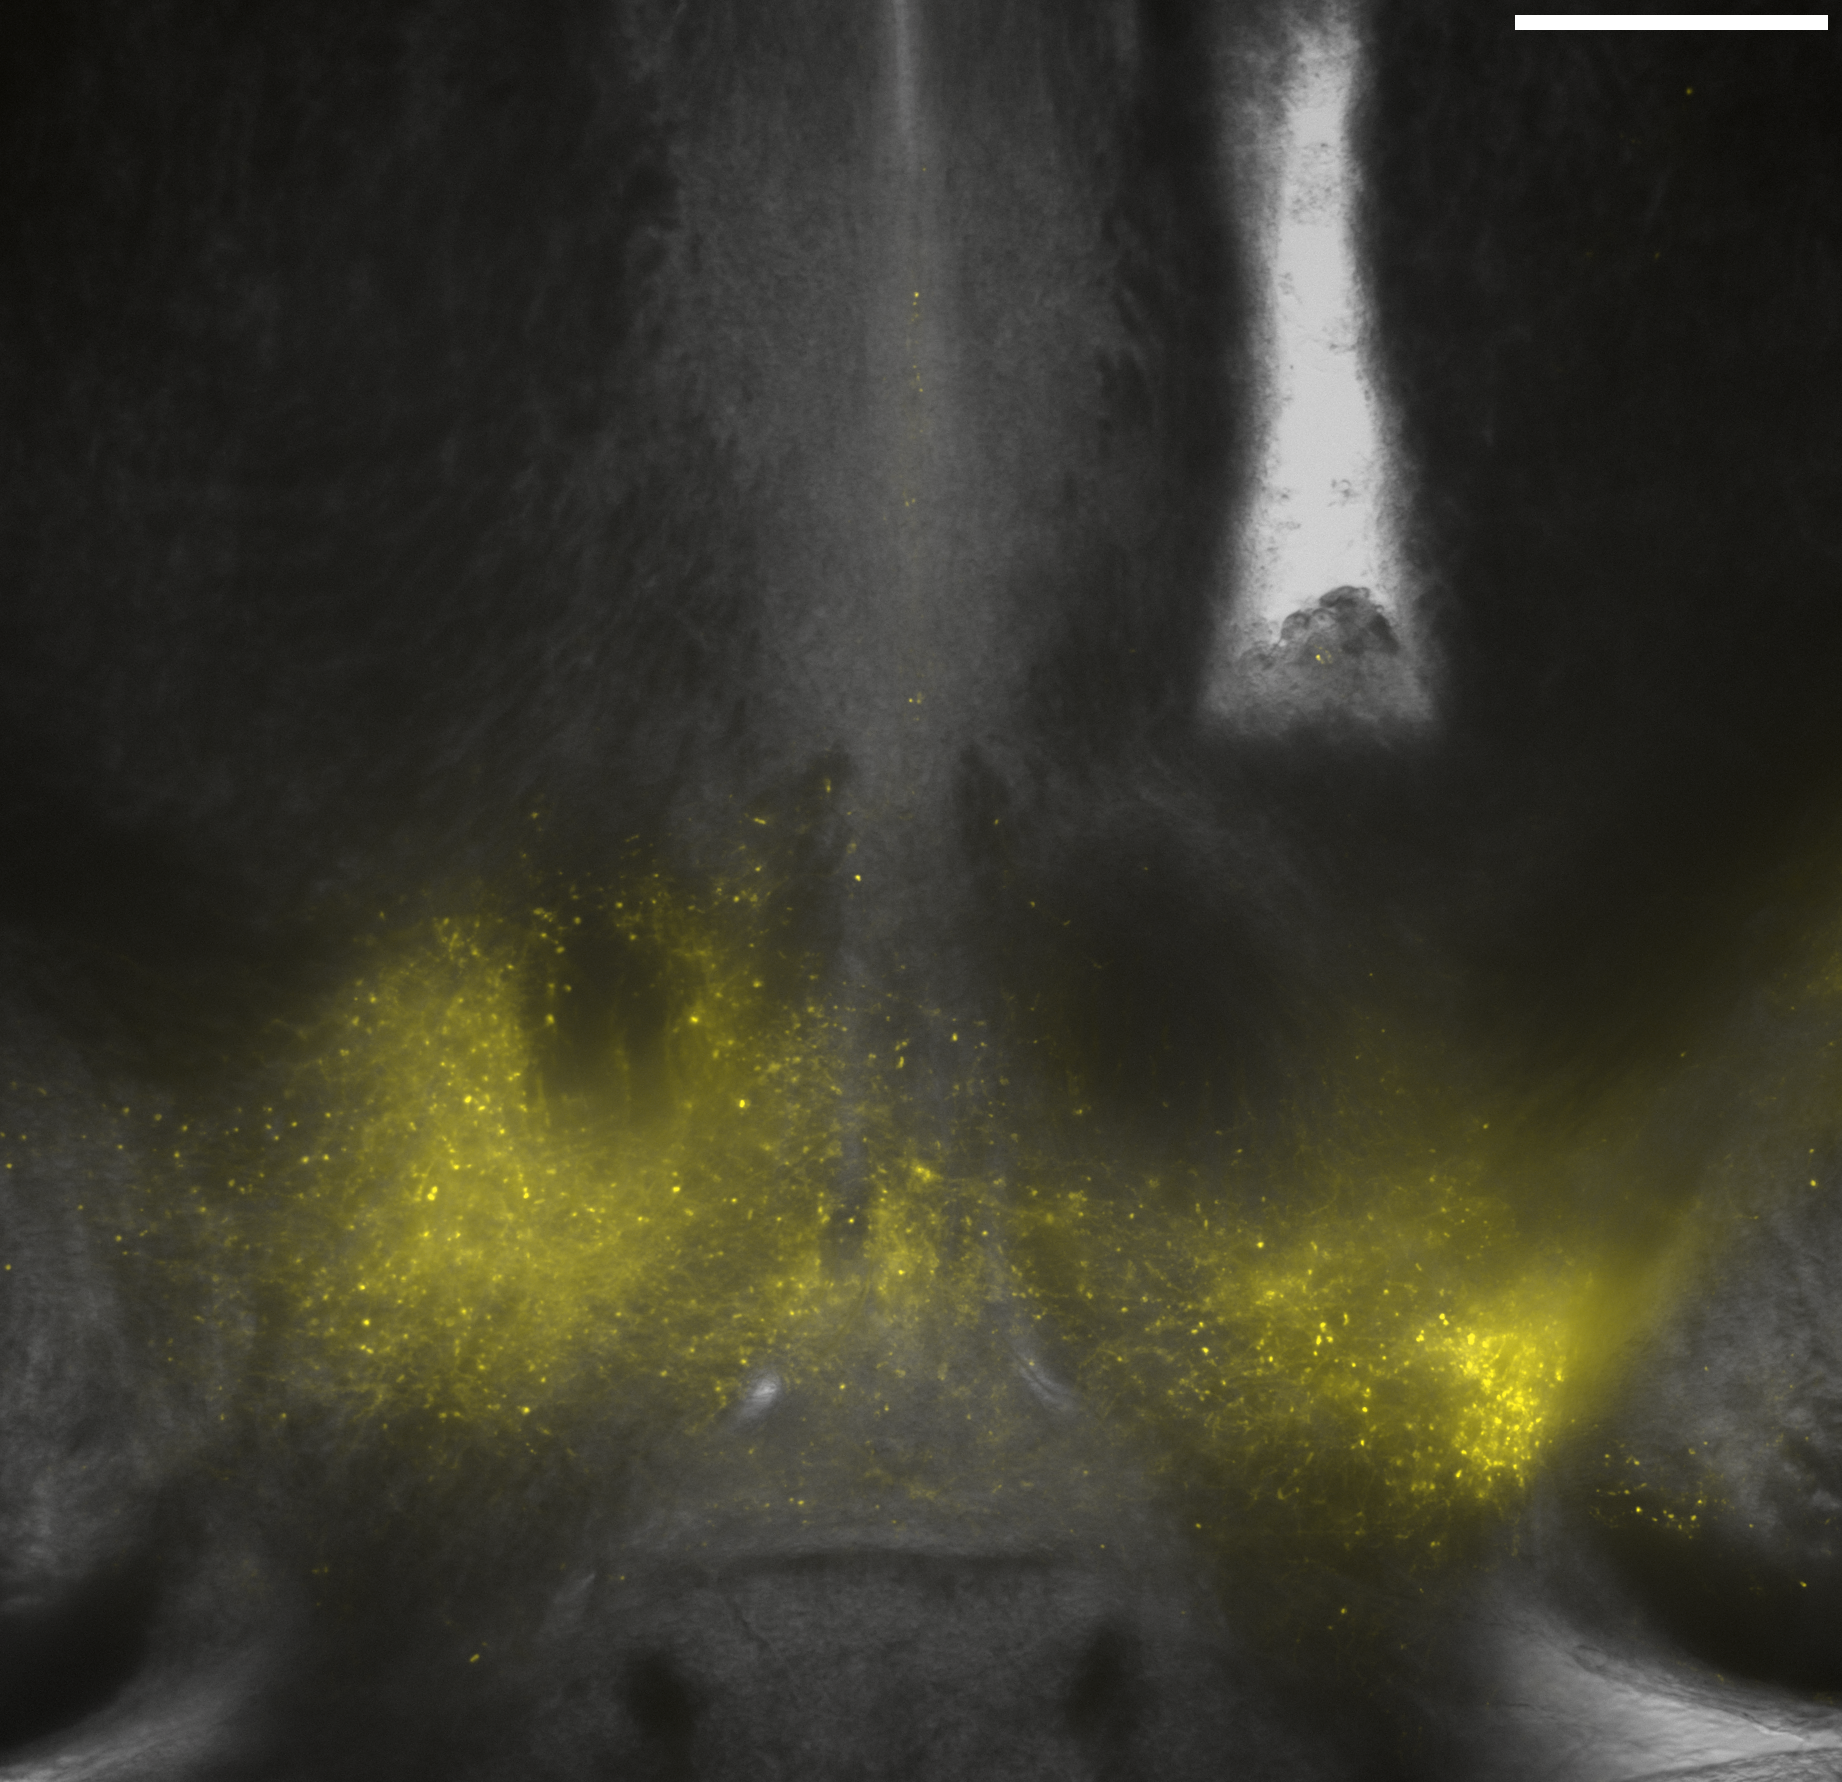
\includegraphics[width=\textwidth]{img/sub-6591_slice-b1_zoom-5_scene-3_transmission-yfp-comb_straight.png}
                \caption{\SI{3.05}{\milli\meter} caudal of Bregma.}
                \label{fig:h6591}
	\end{subfigure}
	\begin{subfigure}{.43\textwidth}
		\centering
		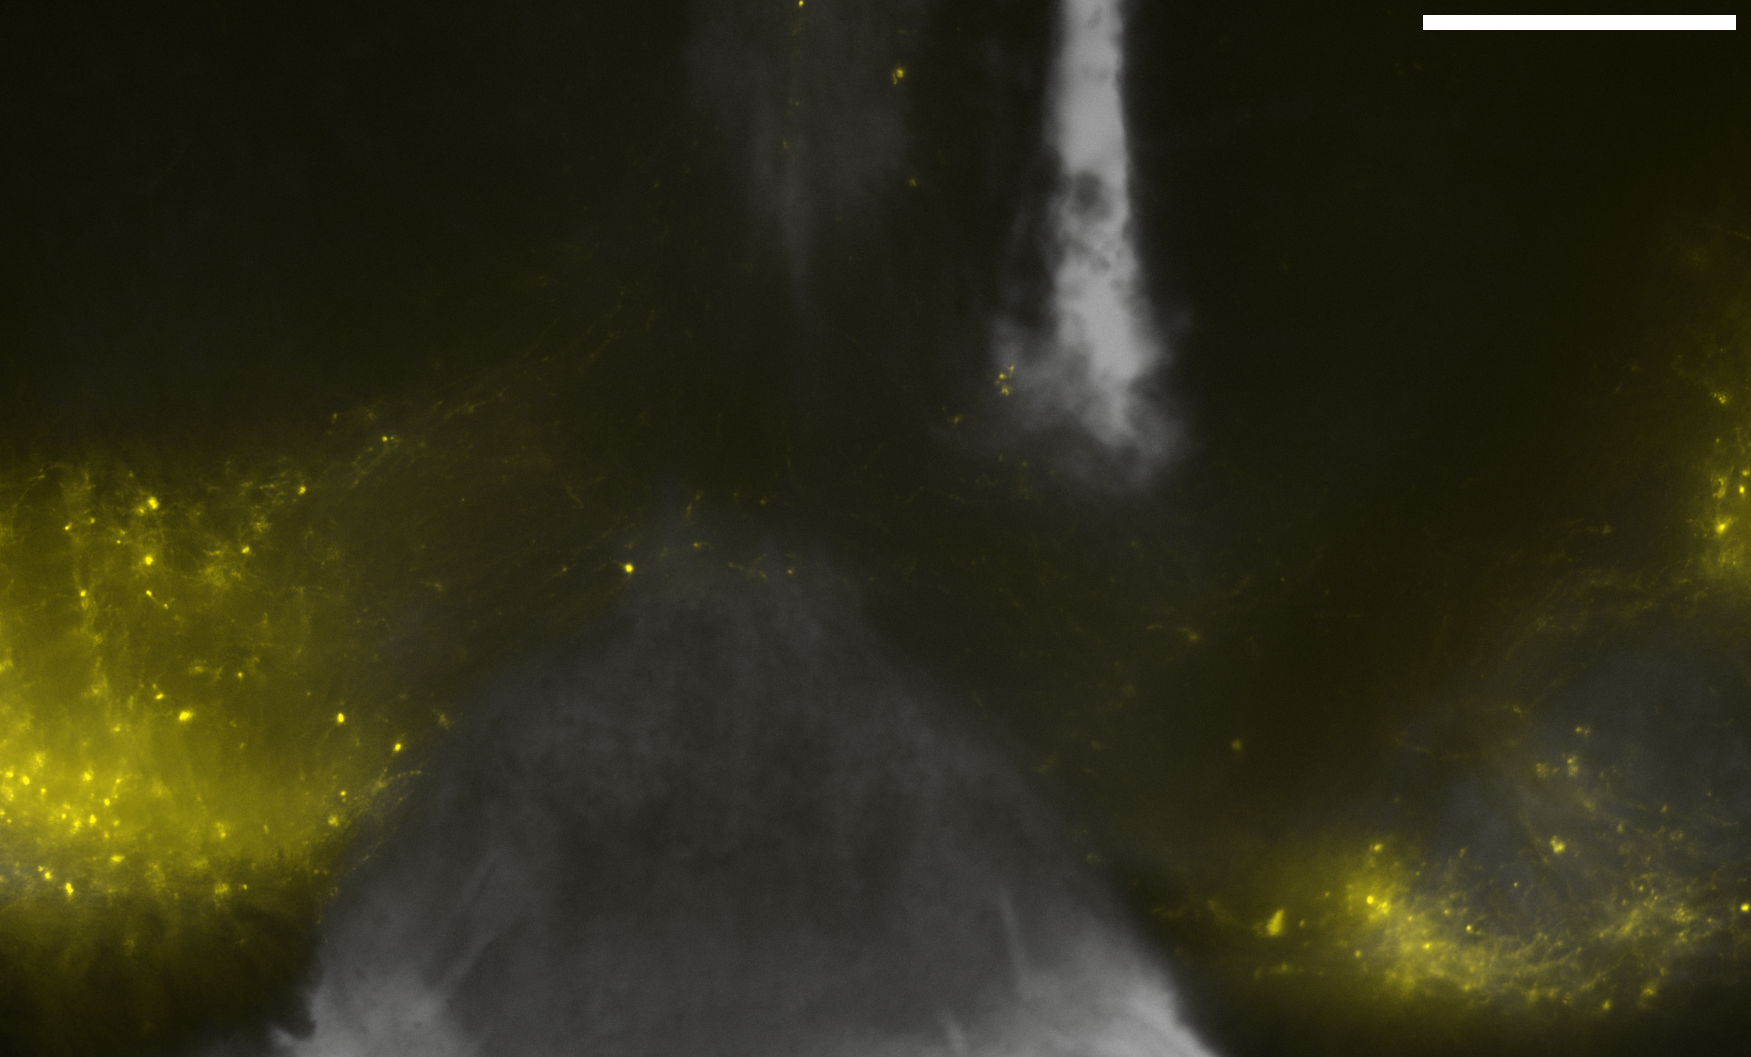
\includegraphics[width=\textwidth]{img/sub-6589_slice-a4_zoom-5_scene-2_transmission-yfp-comb_straight.png}
                \caption{\SI{3.5}{\milli\meter} caudal of Bregma.}
		\label{fig:h6589}
	\end{subfigure}
	\begin{subfigure}{.2728\textwidth}
		\centering
		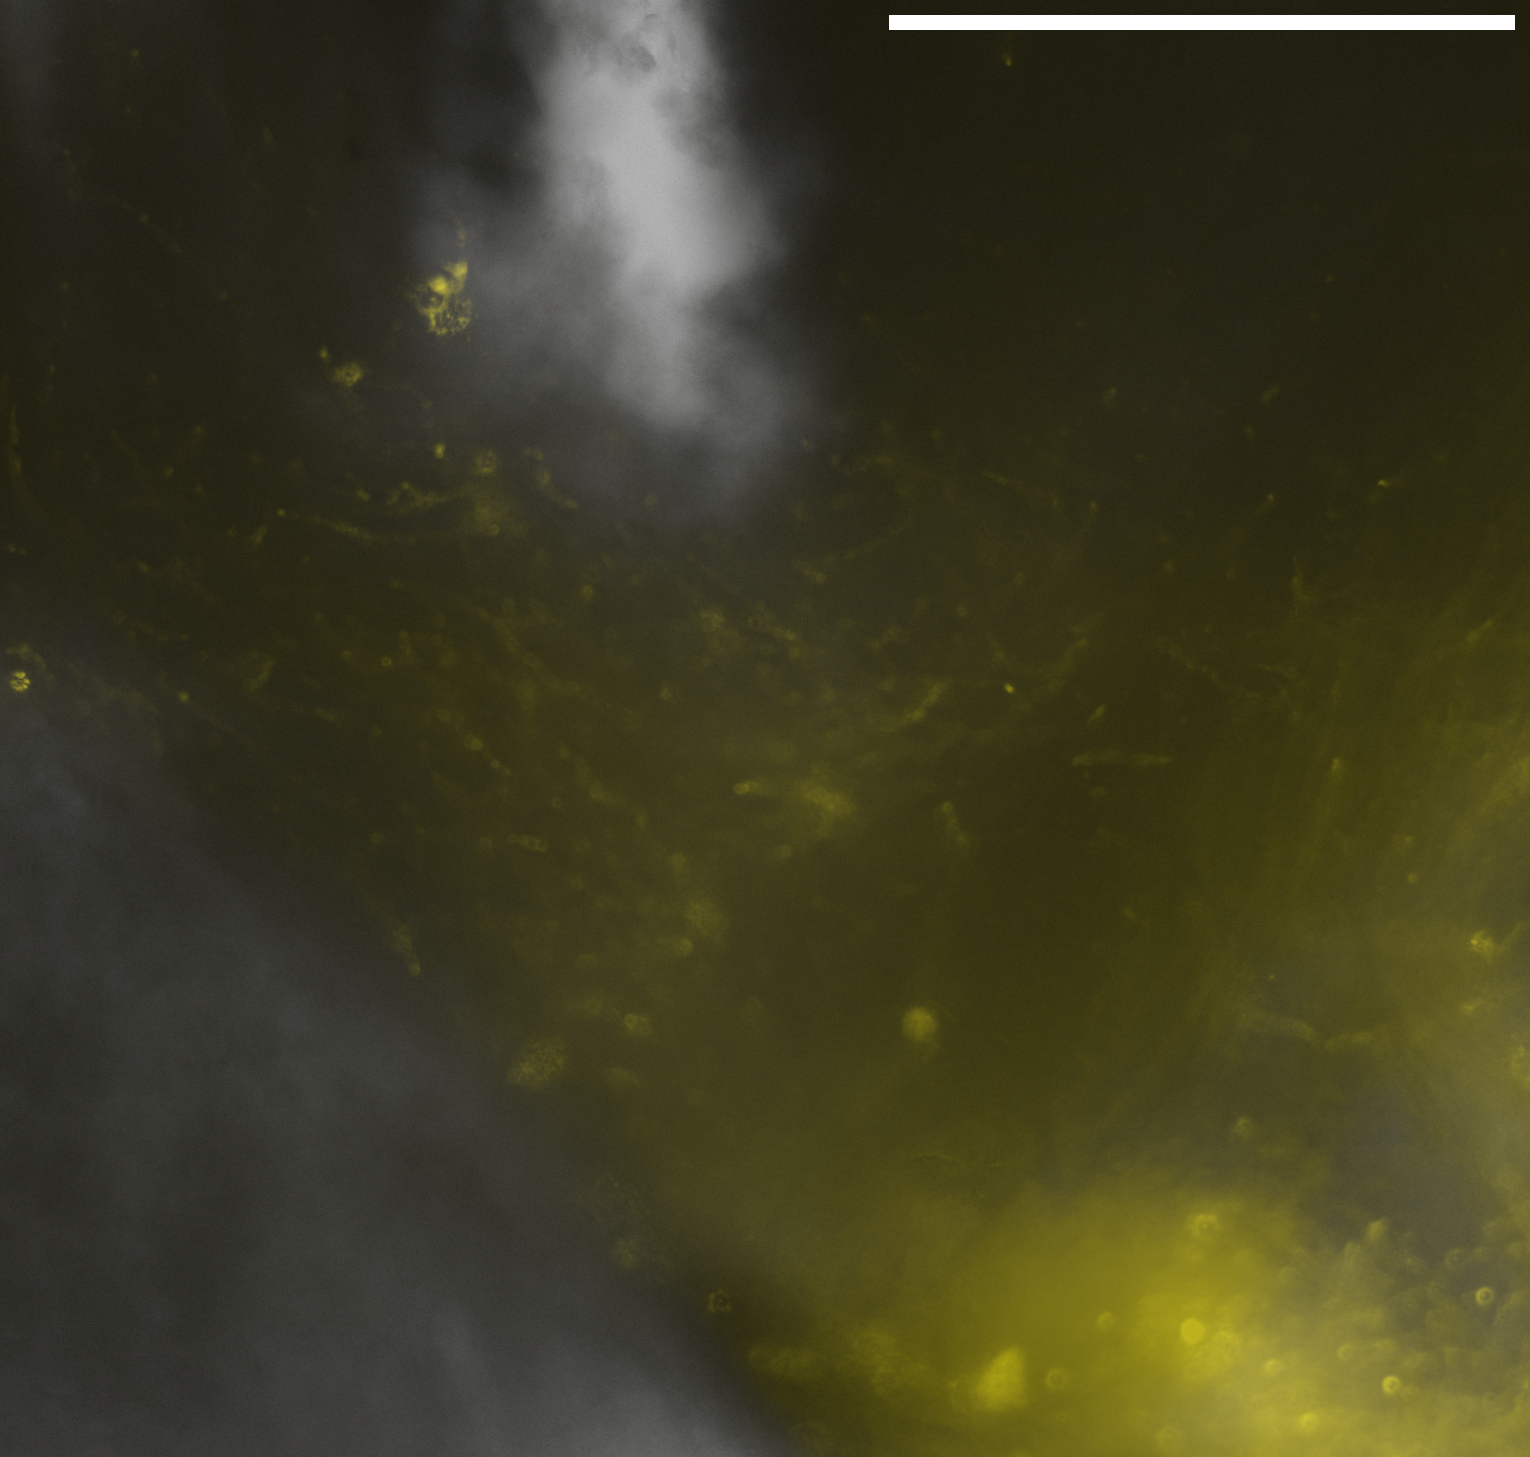
\includegraphics[width=\textwidth]{img/sub-6589_slice-a4_zoom-10_scene-2_transmission-yfp-comb_straight.png}
                \caption{\SI{3.5}{\milli\meter} caudal of Bregma.}
		\label{fig:h6589z}
	\end{subfigure}
        \vspace{-.5em}
	\caption{
		\textbf{Fiber implantation causes strong local cell displacement in the VTA.}
                Depicted are YFP (coexpressed with Channelrhodopsin) fluorescent microscopy images of the VTA, overlain on a corresponding transmission microscopy image of the same focal plane.
                All slices are seen in neurological orientation (the right of the image corresponds to the right of the animal).
                A higher magnification of \textbf{(\subref{fig:h6589})} is depicted in \textbf{(\subref{fig:h6589z})}.
                White bars indicate a scale of \SI{500}{\micro\meter}.
                }
	\label{fig:h}
\end{figure*}

For analysis, the numerous stimulation protocols tested are divided into two categories: phasic stimulation (encompassing protocols where stimulation is delivered in short bursts of up to \SI{1}{\second} in lenght --- \cref{tab:CogP,tab:JPogP}) and block stimulation (where stimulation is delivered in continuous blocks of at least \SI{8}{\second} --- \cref{tab:CogB,tab:CogBr,tab:CogBm,tab:CogMwf}).

The VTA mean t statistic is sensitive to
the stimulation protocol category (\sessionpy{boilerplate.anova(factor='Q("Task Category")')}),
the stimulation target depth (\sessionpy{boilerplate.anova(factor='C(Q("Depth rel. skull [mm]"))')}),
the stimulation target PA coordinates (\sessionpy{boilerplate.anova(factor='C(Q("PA rel. Bregma [mm]"))')}),
and the interaction of the depth and PA target coordinates (\sessionpy{boilerplate.anova(factor='C(Q("Depth rel. skull [mm]")):C(Q("PA rel. Bregma [mm]"))')}).

The break-up by phasic and block stimulation is shown in \cref{fig:mv} and --- accounting for the entire model, including target coordinates --- both levels are significantly different from zero, with
the phasic stimulation level of the variable yielding a p-value of $\sessionpy{boilerplate.posthoc_t('Q("Task Category")[Phasic]')}$,
and the block stimulation level yielding a p-value of $\sessionpy{boilerplate.posthoc_t('Q("Task Category")[Block]')}$.
Upon an investigation of the t-statistic map, phasic stimulation, however, reveals no coherent activation pattern (\cref{fig:phasica}).

The main and interaction effects of the implant coordinate variables are better described categorically than linearly (\cref{fig:mvib,fig:mvip,fig:mvs}).
Consequently, a best-implant group can most reliably be determined based on a categorical classification of implant coordinates.
We classify the implant coordinates into a “best” and a “rejected” group, by k-means clustering the aggregate VTA t-statistic scores into two clusters.
This categorization is highlighted in \cref{fig:mvib,fig:mvip}, and shows different cluster assignments for phasic and block stimulation protocols, with phasic stimulation showing a trend towards more caudal implant coordinates.

For block stimulation, the best implant category group (\cref{fig:filtered}) and the rejected implant category group (\cref{fig:other}) show not only a difference in overall stimulus-evoked signal intensity, but also a difference in efferent distribution, with the rejected implant category more strongly projecting to caudal brain areas.
This distinction specifically arises for implant categorization based on block scan VTA t-statistic means.
It is not as salient or wholly absent if implants are categorized based on VTA activation in both stimulation protocol categories (\cref{fig:occ}) or based on a posteroanterior delimiter (\cref{fig:pcc}).

The activation pattern elicited by block stimulation in the best implant category group shows strong coherent clusters of activation.
The top activation areas are predominantly located in the right hemisphere, with the whole brain parcellation-resolved response showing
highly significant laterality ($p = \sessionpy{boilerplate.lateral('data/l2/alias-block_filtered_controlled/acq-EPI_tstat.nii.gz')}$).
Activation is seen in regions surrounding the stimulation site, such as the ventral tegmental decussation and the interpeduncular nucleus.
The largest activation cluster can be seen in the dopaminergic VTA projection areas, covering subcortical regions in the rostroventral region of the brain (nucleus accumbens, basal forebrain, striatum, and the bed nucleus of the stria terminalis)
Smaller structures in the vicinity of the above regions, such as the anterior commissure and the medial septum, also show activation.

This activation pattern is consistent with published structural projection data (\cref{fig:f}).
At the parcellation level, we see a moderately strong positive correlation between functional activation and strunctural projection (\cref{fig:fcr}), which is weaker at the voxel level (\cref{fig:fcv}).
Qualitatively, a strong overlap of the thresholded activation and projection maps is seen in the midbrain VTA area, while a moderate overlap is observable both in the rostral and caudal projection areas (\cref{fig:ffc}).
Inspecting the the most salient differences (\cref{fig:mff,fig:dff}), we observe that the activation map most notably encompasses additional areas of activation in the contralateral hemisphere (particularly the contralateral nucleus accumbens, with activity extending into the anterior comissure region).
Additionally, there are salient differences around the edges of the ipsilateral striatum, most notably in the claustrum and the fundus of the striatum, extending into close regions such as the anterior comissure.
The pattern of activation, however, appears to encompass all regions with dense structural projections, with areas where structural projection overshoots functional activation being few and dispersed.
These smal clusters amount to weakly negative contrast distributions in regions such as the trunk of the cerebellum, the amygdalopiriform and cortical amygdaloid areas, and a medial subdivision of the cinglate cortex (\cref{fig:dffn}).

We disambiguate VTA transmission from VTA excitability by imaging VTA seed-based functional connectivity, yielding the projection pattern shown in \cref{fig:seed}.
Clusters thus identified are comparatively more sparse than those identified by stimulus-evoked activation, yet follow a similar pattern.
While the top functional connectivity areas are located in the right hemisphere, the whole brain parcellation-resolved response shows
no significant laterality ($p = \sessionpy{boilerplate.lateral('data/seed_l2/alias-block_filtered/acq-EPI_tstat.nii.gz')}$).
Strong activation can be seen in the parcellation regions closely surrounding the seed, such as the ventral tegmental decussation and the closely located interpeduncular nucleus.
Rostrovental dopaminergic projection areas remain prominently featured, including the nucleus accumbens, ventral tenia tecta, stria terminalis, intermediate nucleus of the endopiriform cortex, and the basal forebrain.
A number of caudal projection areas become apparent in this analysis, including a caudal subdivision of the cingulate cortex.
The medial septum, a smaller structure in the vicinity of the striatum, also shows activity.

Stimulation in control animals (which is corrected for in the aforementioned stimulus-evoked analyses) does not show strong dopaminergic activity.
However, sparse grains of regression scores above $t = 3$ can be observed, with the largest cluster in the thalamus, suggesting visual activity (\cref{fig:control_mapa}).
Atlas parcellation (\cref{fig:control_dist}) score distributions do not strongly deviate from zero, with the highest score areas being in the vecinity of the fiber, and thus consistent with VTA heating artefacts (ventral tegmental decussation, interpeduncular nucleus, and the caudal cingulate cortex).
Comparable region t-statistic distributions are also found in the cerebellum (dentate nucleus, lobule 1-3 trunks, and the trunk of the crus).
Overall the whole brain parcellation-resolved response shows
no significant laterality ($p = \sessionpy{boilerplate.lateral('data/seed_l2/alias-block_control/acq-EPI_tstat.nii.gz')}$).

Histological analysis of the targeting site reveals that the optic fiber implant displaces the YFP labelled neurons of the VTA (\cref{fig:h}).
The effect is seen independently of the targeting area or the speed of implant insertion (\SIrange{10}{50}{\micro\meter\per\second}).
Higher magnification (\cref{fig:h6589z}) reveals, however, that labeled filaments remain in the imediate vecinity of the fiber tip.

